%!TEX root = ../main.tex
\usetikzlibrary{arrows}
\subsection{Representation \#2: \acrfull{tf}}

\[
    W(z) = \frac{B(z)}{A(z)} z^{-k} = \frac{b_0 + b_1z_{-1} + b_2z^{-2} + \ldots + b_pz^{-p}}{a_0 + a_1z^{-1} + a_2z^{-2} + \ldots + a_nz^{-n}} z^{-k} 
\]
\vspace{1pt}
\[
     \Sys: y(t) = W(z)u(t)
\]     

The \gls{tf} $W(z)$ is a rational function of \emph{z}: it's a \emph{digital filter}.\\

\begin{remark}[$z$ operator]
    The linear $z$ operator is such that $z^{-1}[x(t)]=x(t-1)$ and $z[x(t)]=x(t+1)$.\\
    From now on the "$[\cdot]$" will be \textbf{omitted} for simplicity.
\end{remark}

%Now it's trivial to move from T.F. representation to a time domain description of the system.

\begin{example}
    \begin{align*}
    \Sys: \quad
        & y(t) = \underbrace{\begin{bmatrix}
            \frac{1+\frac{1}{2}z^{-1}}{2+\frac{1}{3}z^{-1}+\frac{1}{4}z^{-2}} z^{-1}
        \end{bmatrix}}_{W(z)} u(t) \\
        & 2y(t) + \frac{1}{3}y(t-1) + \frac{1}{4}y(t-2) = u(t-1) + \frac{1}{2}u(t-2) \\
        & y(t) = \underbrace{-\frac{1}{6}y(t-1) - \frac{1}{8}y(t-2)}_\text{recursive part} + \underbrace{\frac{1}{2}u(t-1) + \frac{1}{4}u(t-2)}_\text{past inputs}
    \end{align*}

\end{example}
\begin{remark}[IRR and FIR filters]
\hfill \break 
    $\displaystyle W(z) = \frac{z^{-1}}{1 + \frac{1}{3}z^{-1}}$ is an IIR (\emph{Infinite Impulse Response}) filter since it has the recursive part because of the presence of \emph{poles} in $W(z)$.\\
    $\displaystyle W(z) = z^{-1} + \frac{1}{2}z^{-2} + \frac{1}{4}z^{-3}$ is a FIR (\emph{Finite Impulse Response}) filter since it depends only on a \emph{finite} sequence of past inputs.
\end{remark}

\begin{remark}[Strictly proper systems]
    Notice that for strictly proper systems the delay of $W(z)$ is $k \ge 1$, or, equivalently, the order of the numerator of $W(z)$ is strictly smaller than the order of the numerator of $W(z)$.
    \begin{figure}[H]
        \begin{minipage}[t]{0.5\textwidth}
            \centering
            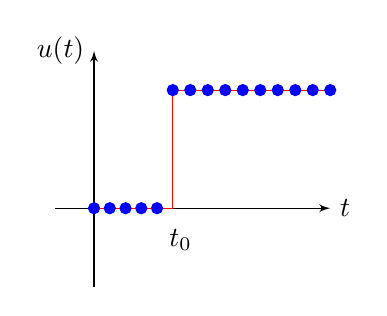
\begin{tikzpicture}[node distance=2.5cm,auto,>=latex']
                \draw[->] (-0.5,0) -- (3,0) node[right] {$t$};
                \draw[->] (0,-1) -- (0,2) node[left] {$u(t)$};
                \draw[domain=0:1,smooth,variable=\x,red] plot ({\x},{0});
                \draw[domain=1:3,smooth,variable=\x,red] plot ({\x},{1.5});
                \draw[red] (1,0) -- (1,1.5);
                \draw[mark=*, mark options={fill=blue},blue,samples=5,domain=0:0.8,only marks,variable=\x] plot ({\x},{0});
                \draw[mark=*, mark options={fill=blue},blue,samples=10,domain=1:3,only marks,variable=\x] plot ({\x},{1.5});
                \node at (1.1,-0.4) {$t_0$};
            \end{tikzpicture}
        \end{minipage}
        \begin{minipage}[t]{0.5\textwidth}
            \centering
            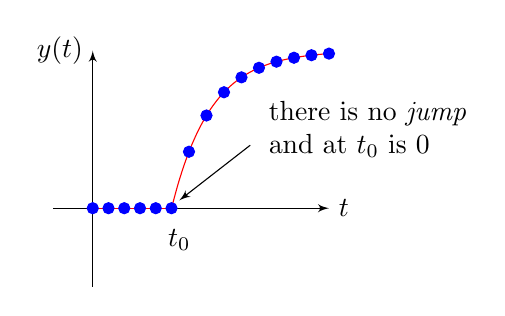
\begin{tikzpicture}[node distance=2.5cm,auto,>=latex']
                \draw[->] (-0.5,0) -- (3,0) node[right] {$t$};
                \draw[->] (0,-1) -- (0,2) node[left] {$y(t)$};
                \draw[domain=0:1,smooth,variable=\x,red] plot ({\x},{0});
                \draw[domain=1:3,smooth,variable=\x,red] plot ({\x},{2*(1-e^(-(\x-1)*2))});
                \draw[mark=*, mark options={fill=blue},blue,samples=5,domain=0:0.8,only marks,variable=\x] plot ({\x},{0});
                \draw[mark=*, mark options={fill=blue},blue,samples=10,domain=1:3,only marks,variable=\x] plot ({\x},{2*(1-e^(-(\x-1)*2))});
                \node at (1.1,-0.4) {$t_0$};
                \node[align=left] at (3.5,1) {there is no \emph{jump}\\ and at $t_{0}$ is 0};
                \draw[->] (2,0.8) -- (1.1,0.1);
            \end{tikzpicture}
        \end{minipage}
    \end{figure}
\end{remark}

\subsection{Representation \#3: Convolution of the input with the \acrfull{ir}}
The third way to represent a system is through the \emph{convolution} of the input with the \emph{\acrfull{ir}}.\\
\begin{definition}[\acrlong{ir}]
    In the discrete time domain, the \acrlong{ir} of a filter $W(z)$ is $y(t) = W(z)u(t)$ where the input $\omega(t)$ is an impulse (i.e. $u(t)=0$ everywhere except from $t=0$ where $u(t=0)=0$).
    \[
    \omega(t)=\{\omega(0), \omega(1), \omega(2), \cdots\}
    \]
\end{definition}

\begin{figure}[H]
    \begin{minipage}[t]{0.5\textwidth}
        \centering
        \begin{tikzpicture}[node distance=2.5cm,auto,>=latex']
            \draw[->] (-0.5,0) -- (3,0) node[right] {$t$};
            \draw[->] (0,-1) -- (0,2) node[left] {$u(t)$};
            \draw[domain=-0.3:0,smooth,variable=\x,red] plot ({\x},{0});
            \draw[domain=0:0.2,smooth,variable=\x,red] plot ({\x},{1.5});
            \draw[domain=0.2:2.5,smooth,variable=\x,red] plot ({\x},{0});
            \draw[mark=*, mark options={fill=blue},blue,samples=1,domain=0:0.00001,only marks,variable=\x] plot ({\x},{1.5});
            \draw[mark=*, mark options={fill=blue},blue,samples=5,domain=0.4:2.5,only marks,variable=\x] plot ({\x},{0});
        \end{tikzpicture}
        \caption*{Impulse in input}
    \end{minipage}
    \begin{minipage}[t]{0.5\textwidth}
        \centering
        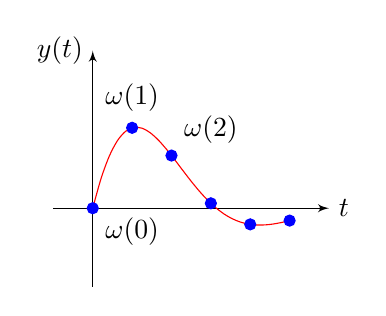
\begin{tikzpicture}[node distance=2.5cm,auto,>=latex']
            \draw[->] (-0.5,0) -- (3,0) node[right] {$t$};
            \draw[->] (0,-1) -- (0,2) node[left] {$y(t)$};
            \draw[domain=0:2.5,smooth,variable=\x,red] plot ({\x},{2*sin(\x*180/3.14*2)*e^(-\x)});
            \draw[mark=*, mark options={fill=blue},blue,samples=6,domain=0:2.5,only marks,variable=\x] plot ({\x},{2*sin(\x*180/3.14*2)*e^(-\x)});
            \node at (0.5,-0.3) {$\omega(0)$};
            \node at (0.5,1.4) {$\omega(1)$};
            \node at (1.5,1.0) {$\omega(2)$};
        \end{tikzpicture}
        \caption*{\gls{ir} in output}
    \end{minipage}
\end{figure}

\textbf{Note} if the system is strictly proper then $\omega(0) = 0$.

It can be proven that the input-output relationship from $u(t)$ to $y(t)$ can be written as
\[ y(t) = \omega(0) u(t) + \omega(1) u(t-1) + \omega(2) u(t-2) + \cdots
        = \sum_{k=0}^{\infty} \omega(k) u(t-k) \]
From this, it is clear that $y(t)$ is the \emph{convolution} of the \gls{ir} with the input signal.

%naming transformations
\newcommand\nameeq[2]{\text{\qquad #2:}&&#1&&\phantom{\text{#2:}}}

\section{Transformations between representations}
It is possible translate each representation into another one. Therefore, there are six possible transformations between the three representations.
\begin{figure}[H]
    \centering
    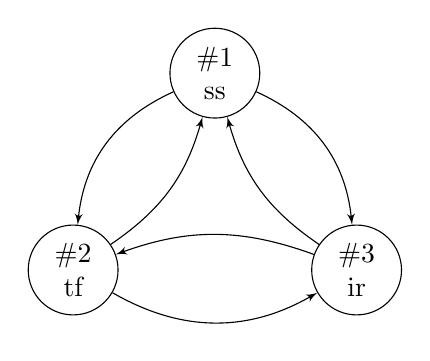
\begin{tikzpicture}[node distance=2.5cm,auto,>=latex']
        \node (n1) [draw, circle, align=center]{\#1\\\acrshort{ss}};
        \node (n2) [draw, circle, align=center, below of=n1, xshift=-1.8cm] {\#2\\\gls{tf}};
        \node (n3) [draw, circle, align=center, below of=n1, xshift= 1.8cm] {\#3\\\gls{ir}};

        \draw[->] (n1) edge[bend right] (n2);
        \draw[->] (n2) edge[bend right] (n3);
        \draw[->] (n1) edge[bend left] (n3);
        \draw[->] (n2) edge[bend right=20] (n1);
        \draw[->] (n3) edge[bend right=20] (n2);
        \draw[->] (n3) edge[bend left=20] (n1);
    \end{tikzpicture}
    \caption*{Transformations between representations}
\end{figure}

\subsection{\acrlong{ss} to \acrlong{tf}}
Consider a strictly proper system with the following \gls{ss} representation:
\[
\Sys: 
\begin{cases}
    x(t+1) = F x(t) + G u(t)\\
    y(t) = H x(t) + \cancelto{0}{D u(t)}\\
\end{cases}
\Rightarrow
\begin{cases}
    x(t+1) = F x(t) + G u(t)\\
    y(t) = H x(t)\\
\end{cases}
\]
From the system we get
\[ z x(t) = F x(t) + G u(t) \Rightarrow x(t) = (zI - F)^{-1} G u(t) \]
\[ \Rightarrow y(t) = H (zI - F)^{-1} G \cdot u(t) \]
Thus, the \acrlong{tf} is
\begin{flalign}
    \nameeq{W(z) = H(zI - F) ^ {-1} G}{\gls{ss}\textrightarrow\gls{tf}}\label{t1}
\end{flalign}

\begin{example}{Consider the following SISO system of order $n=2$:}
\begin{align*}
    F = \begin{bmatrix}
        1 & 0\\
        \frac{1}{2} & 2\\
    \end{bmatrix}
    &&
    G = \begin{bmatrix}
        1\\
        1\\
    \end{bmatrix}
    &&
    H = \begin{bmatrix}
        1 & 0\\
    \end{bmatrix}
    &&
    D = 0
\end{align*}

Using the transformation \ref{t1}:
\vspace{-10pt}

\begin{align*}
W(z) &=
\begin{bmatrix}
    1 & 0\\
\end{bmatrix}
\left( \begin{bmatrix}
    z & 0\\
    0 & z\\
\end{bmatrix}
-
\begin{bmatrix}
    1 & 0 \\
    \frac{1}{2} & 2\\
\end{bmatrix}\right)^{-1}
\begin{bmatrix}
    1\\
    1\\
\end{bmatrix}
= \begin{bmatrix}
    1 & 0\\
\end{bmatrix}
\begin{bmatrix}
    z-1 & 0\\
    -\frac{1}{2} & z-2\\
\end{bmatrix}^{-1}
\begin{bmatrix}
    1\\
    1\\
\end{bmatrix}\\
&= \begin{bmatrix}
    1 & 0\\
\end{bmatrix}
\frac{1}{(z-1)(z-2)}
\begin{bmatrix}
    z-2 & 0\\
    \frac{1}{2} & z-1\\
\end{bmatrix}
\begin{bmatrix}
    1\\
    1\\
\end{bmatrix}
=
\frac{1}{(z-1)(z-2)}
\begin{bmatrix}
    z-2 & 0\\
\end{bmatrix}
\begin{bmatrix}
    1\\
    1\\
\end{bmatrix}\\
&=
\frac{\cancel{z-2}}{(z-1)\cancel{(z-2)}} = \frac{1}{z-1} = \frac{1}{1-z^{-1}} z^{-1}
\end{align*}
Notice that, due to \textbf{cancellation of singularities}, in this case we only have one pole, but the system is of order two; this comes from the fact that part of the system is \emph{non observable}.\\
Alternatively, it could be noted that $\{F, G, H, D\}$ corresponds to the following system:
    \[
    \Sys: 
        \begin{cases}
            x_1(t+1) = x_1(t) + u(t) \\
            x_2(t+1) = \frac{1}{2} x_1(t) + 2x_2(t) + u(t) \\
            y(t) = x_1(t)
        \end{cases}
    \Rightarrow
        \begin{cases}
            zx_1(t) = x_1(t) + u(t) \\
            zx_2(t) = \frac{1}{2} x_1(t) + 2x_2(t) + u(t) \\
            y(t) = x_1(t)
        \end{cases}    
    \]
From the first equation we have that $x_{1}(t)=\frac{1}{z-1}u(t)$ and substituting it to the third one we obtain the same result: $y(t)=x_{1}(t)=\frac{1}{z-1}u(t) \Rightarrow W(z)=\frac{1}{1-z^{-1}} z^{-1}$     

\end{example}

\subsection{\acrlong{tf} to \acrlong{ss}}
This conversion is not very used in practice and it is called the \emph{realization} of a \acrlong{tf} into a \acrlong{ss} system.

\textbf{Issue}: the \acrlong{ss} representation is not unique! Thus from a single \acrlong{tf} we can get infinite different equivalent \acrlong{ss} models.

\subsubsection{Control realization}

We assume that the system is \textbf{strictly proper} and that the denominator is \textbf{monic} (i.e. $a_0=1$).
\[ W(z) = \frac{b_0 z^{n-1} + b_1 z^{n-2} + \dots + b_{n-1}}{z^n + a_1 z^{n-1} + a_2 z^{n-2} + \dots + a_n} \]

The formula for the control realization of $W(z)$ is
\begin{flalign}
\nameeq{
    F = \begin{bmatrix}
        0 & 1 & 0 & \cdots & 0\\
        0& 0 & 1 & \ddots & \vdots \\
        \vdots & \vdots & \ddots & \ddots & 0\\
        0 & 0 & \cdots & 0 & 1\\
        -a_n & -a_{n-1} & \multicolumn{2}{c}{\cdots} & -a_1\\
    \end{bmatrix}
    &&
    G = \begin{bmatrix}
        0\\
        0\\
        0\\
        \vdots\\
        1\\
    \end{bmatrix}
    &&
    H = \begin{bmatrix}
        b_{n-1} & b_{n-2} & \cdots & b_0\\
    \end{bmatrix}
    &&
    D = 0
    }{\gls{tf}\textrightarrow\gls{ss}}\label{t2}
\end{flalign}
\begin{example}
    Consider the following \acrlong{tf}:
    \[ W(z) = \frac{2z^2 + \frac{1}{2}z + \frac{1}{4}}{z^3 + \frac{1}{4}z^2 + \frac{1}{3}z + \frac{1}{5}} \]
    Applying the transformation \ref{t2}, the control realization is:
    \begin{align*}
        F = \begin{bmatrix}
            0 & 1 & 0\\
            0 & 0 & 1\\
            -\frac{1}{5} & -\frac{1}{3} & -\frac{1 }{4}\\
        \end{bmatrix}
        &&
        G = \begin{bmatrix}
            0\\
            0\\
            1\\
        \end{bmatrix}
        &&
        H = \begin{bmatrix}
            \frac{1}{4} & \frac{1}{2} & 2\\
        \end{bmatrix}
        &&
        D = 0
    \end{align*}
\end{example}

\subsection{\acrlong{tf} to \acrlong{ir}}
To get the \gls{ir} from a \acrlong{tf} $W(z)$ is sufficient to make the $\infty$-long division between the numerator and denominator of $W(z)$.
\begin{flalign}
\nameeq{\omega(t)= 
    \begin{cases}
        e_{t} \qquad \text{if $t \ge 1$}\\
        0     \qquad \text{ if $t=0$ (and $W(z)$ is strictly-proper)}
    \end{cases}
    }{\gls{tf}\textrightarrow\gls{ir}}\label{t3}
\end{flalign}
\qquad where $e_{t}$ are the coefficients of 
\[E(z) = e _{1}z^{-1} + e_{2}z^{-2} + \cdots = \sum_{t=1}^{\infty} e_{t}z^{-t}\]
\qquad which is the \emph{remainder} of the $\infty$-long division.
\begin{example}
    Consider the following \acrlong{tf}:
    \[ W(z) = \frac{1}{z-\frac{1}{2}} = \frac{z^{-1}}{1-\frac{1}{2}z^{-1}}
        \stackrel{\text{$\infty$-long div.}}{=} 0 z^{-0} + 1 z^{-1} + \frac{1}{2}z^{-2} + \frac{1}{4}z^{-3} + \cdots \]
    Applying the transformation \ref{t3} the \gls{ir} is $\omega(0) = 0$, $\omega(1) = 1$, $\omega(2) = \frac{1}{2}$, $\omega(3) = \frac{1}{4}$, $\dots$
    Thus $\omega(0)=0$ and $\omega(t) = \frac{1}{2^{t-1}} \quad \forall t \ge 1$
    %\\and $y(t)$ is the convolution of $u(t)$ with the \gls{ir} $w(t)$, indeed: 
    %\[
    %    y(t)=W(z)u(t)=\omega(0)u(0)+\omega(1)u(1)+\cdots = \sum_{k=0}^{\infty}\omega(t)u(t-k)
    %\]

    In this case there is also a quicker way
    \[ y(t) = \frac{z^{-1}}{1-\frac{1}{2}z^{-1}} u(t) = \left( z^{-1} \frac{1}{1-\frac{1}{2}z^{-1}} \right) u(t) \]
    Remembering that for \emph{geometric series} we have \[ \sum_{k = 0}^{\infty} a^k = \frac{1}{1-a} \text{ if } |a| < 1 \]
    We can rewrite $y(t)$ as follows
    \[ y(t) = \left( z^{-1} \sum_{k=0}^{\infty} \left( \frac{1}{2} z^{-1} \right)^{k} \right) u(t) = \left( 0 + 1 z^{-1} + \frac{1}{2}z^{-2} + \frac{1}{4}z^{-3} + \cdots \right) u(t) \]
\end{example}

\subsection{\acrlong{ir} to \acrlong{tf}}
\begin{definition}
    Given a discrete-time signal $s(t)$ such that $\forall t < 0: s(t) = 0$, its \emph{Z-Transform} is defined as
    \[ \mathcal{Z} \left( s(t) \right) = \sum_{t = 0}^{\infty} s(t) z^{-t} \]
\end{definition}
Given this, it can be proven that
\begin{flalign}
\nameeq{W(z) = \mathcal{Z}\left( \omega(t) \right) = \sum_{t = 0}^{\infty} \omega(t) z^{-t}}{\gls{tf}\textrightarrow\gls{ir}}\label{t4}
\end{flalign}
This means that the \textbf{\acrlong{tf} of a system} is the $\mathcal{Z}$-transform of a special signal, $\omega(t)$, that is the \acrlong{ir} of the system.

\begin{remark}
    This formula cannot be used in practice to transform an \gls{ir} representation to a \gls{tf} representation.
    This is because we need infinite points of the \acrlong{ir}, and it must be available \emph{noise-free}.
    Thus, this transformation is only theoretical.
\end{remark}

\subsection{\acrlong{ss} to \acrlong{ir}}
Consider the following \acrlong{ss} model, with initial conditions $x(0) = 0$ and $y(0) = 0$
\[
    \Sys: 
    \begin{cases}
        x(t+1) = F x(t) + G u(t)\\
        y(t) = H x(t)\\
    \end{cases}
\]
"Running the simulation of the system", we have that
\begin{align*}
    x(1) &= \cancelto{0}{F x(0)} + G u(0) = G u(0)\\
    y(1) &= H x(1) = H G u(0)\\
         &\Downarrow\\
    x(2) &= F x(1) + G u(1) = F G u(0) + G u(1)\\
    y(2) &= H x(2) = H F G u(0) + H G u(1)\\
         &\Downarrow\\
    x(3) &= F x(2) + G u(2) = F^2 G u(0) + F G u(1) + G u(2)\\
    y(3) &= H x(3) = H F^2 G u(0) + H F G u(1) + H G u(2)\\
         &\vdots
\end{align*}
This can be generalized to
\[ y(t) = 0 u(t) + H G u(t-1) + H F G u(t-2) + H F^2 G u(t-3) + \cdots \]
Recalling that 
\[ y(t) = \omega(0) u(t) + \omega(1) u(t-1) + \omega(2) u(t-2) + \omega(3) u(t-3) + \cdots \]
we deduce that $\omega(0)=0,\, \omega(1)=H G,\, \omega(2)=H F G,\, \omega(3)= H F^2 G,\, \dots $\\
Thus, the \acrlong{ir} is
\begin{flalign}
\nameeq{
    \omega(t) =
    \begin{cases}
        0 \text{           if } t = 0\\
        H F^{t-1} G \text{ if } t > 0
    \end{cases}
}{\gls{ss}\textrightarrow\gls{ir}}\label{t5}
\end{flalign}
